%% ****** Start of file apstemplate.tex ****** %
%%
%%
%%   This file is part of the APS files in the REVTeX 4 distribution.
%%   Version 4.1r of REVTeX, August 2010
%%
%%
%%   Copyright (c) 2001, 2009, 2010 The American Physical Society.
%%
%%   See the REVTeX 4 README file for restrictions and more information.
%%
%
% This is a template for producing manuscripts for use with REVTEX 4.0
% Copy this file to another name and then work on that file.
% That way, you always have this original template file to use.
%
% Group addresses by affiliation; use superscriptaddress for long
% author lists, or if there are many overlapping affiliations.
% For Phys. Rev. appearance, change preprint to twocolumn.
% Choose pra, prb, prc, prd, pre, prl, prstab, prstper, or rmp for journal
%  Add 'draft' option to mark overfull boxes with black boxes
%  Add 'showpacs' option to make PACS codes appear
%  Add 'showkeys' option to make keywords appear
\documentclass[footinbib,aps,prl,superscriptaddress]{revtex4-1}
%\documentclass[aps,prl,preprint,superscriptaddress]{revtex4-1}
%\documentclass[aps,prl,reprint,groupedaddress]{revtex4-1}

% You should use BibTeX and apsrev.bst for references
% Choosing a journal automatically selects the correct APS
% BibTeX style file (bst file), so only uncomment the line
% below if necessary.
%\bibliographystyle{apsrev4-1}

\usepackage{amsmath}
\usepackage{amssymb}
\usepackage{graphicx}
\graphicspath{{../Graphics/Supplement_Graphics/}}
\usepackage{gensymb}


\begin{document}

% Use the \preprint command to place your local institutional report
% number in the upper righthand corner of the title page in preprint mode.
% Multiple \preprint commands are allowed.
% Use the 'preprintnumbers' class option to override journal defaults
% to display numbers if necessary
%\preprint{}

%Title of paper
\title{Supplemental Information for ``Polarization state generation and measurement in parallel with a single metasurface"}


% repeat the \author .. \affiliation  etc. as needed
% \email, \thanks, \homepage, \altaffiliation all apply to the current
% author. Explanatory text should go in the []'s, actual e-mail
% address or url should go in the {}'s for \email and \homepage.
% Please use the appropriate macro foreach each type of information

% \affiliation command applies to all authors since the last
% \affiliation command. The \affiliation command should follow the
% other information
% \affiliation can be followed by \email, \homepage, \thanks as well.
%\author{Noah A. Rubin}
%\author{Federico Capasso}
%\email[]{capasso@seas.harvard.edu}
%\homepage[]{Your web page}
%\thanks{}
%\altaffiliation{}
%\affiliation{John A. Paulson School of Engineering and Applied Sciences, Harvard University, Cambridge, MA 02138, USA}

%Collaboration name if desired (requires use of superscriptaddress
%option in \documentclass). \noaffiliation is required (may also be
%used with the \author command).
%\collaboration can be followed by \email, \homepage, \thanks as well.
%\collaboration{}
%\noaffiliation

\date{\today}

% insert suggested PACS numbers in braces on next line
%\pacs{}
% insert suggested keywords - APS authors don't need to do this
%\keywords{}

%\maketitle must follow title, authors, abstract, \pacs, and \keywords
\maketitle

% body of paper here - Use proper section commands
% References should be done using the \cite, \ref, and \label commands
%\frame{
\includegraphics[width=\textwidth]{Fig1.eps}}


\tableofcontents


\section{Optimization: Details and Discussion}

\subsection{Schematic of procedure}

\subsection{Fabrication of Structures}

\subsection{FDTD Simulation of Designed Gratings}

\subsection{Effect of the Fabrication Imperfections on Produced Polarization Ellipses}

\subsection{Limits of the Scheme}

\section{Metasurface Polarimetry}

In this section we discuss the use of a metasurface polarization grating as a full-Stokes polarimeter, that is, as a sensor enabling the detection of incident polarization state based on the intensities measured on each of the four channels. These channels are the beams diffracted into the $m = -2$, $-1$, $+1$, and $+2$ diffraction orders, after passing through a linear polarizer oriented at $45\degree$.

\subsection{Details of Optical Setup}

Of particular importance in polarimetry is the quality of polarization optics used in calibration. After all, uncertainty about the polarizations used for calibration degrades the ultimate accuracy of any calibrated polarimeter. Of course, absolute polarization references are few-and-far-between \cite{Snik2014}. Perhaps the only absolute polarization state references that exist are those of atomic transitions, constrained by quantum mechanical selection rules to take on a certain polarization state. Thus, in the field of polarimetry, polarimeters are often assessed by comparison with pre-established polarimeters (as we have done in the main text).

Nevertheless, we must establish some certainty about the polarization optics we use.

\subsubsection{Polarizers}

Film-based polarizers are especially tempting, particularly in the visible region --- by far, these are the least expensive options and lend themselves to mass production. Take, for example, a commercially available film polarizer from the vendor ThorLabs (part no. LPVISE100-A). The part specifications claim an intensity extinction ratio of approximately 8000. Given this, we initially anticipated that these would be sufficient, given our needs. However, upon testing, we have found that the intensity extinction ratio of these film polarizers is often well below 1000, sometimes on the order of hundreds. For polarimetry, especially the presently considered metasurface-based polarimeter, this is a significant problem. The fundamental quantity is the electric field, which goes as the square root of the intensity. If the intensity extinction ratio is on the order of hundreds, the electric field extinction ratio is only on the order of tens. This is not acceptable.

Whereas film polarizers rely on inherent material dichroism, a second polarizer strategy relies on birefringent crystalline materials. Glan-Thompson (and Glan-Taylor) polarizers sandwich two birefringent crystals together in a beamsplitter-like configuration. The two are cut so that one linear polarization transmits through relatively unattenuated, while the other totally internally reflects. Since the polarizing mechanism here uses total internal reflection rather than some property subject to an artificial medium, the extinction ratios may be much higher. For instance, our primary polarizer used in all the polarimetry and polarization state measurements (ThorLabs part no. GTH5M-A) has a specified intensity extinction ratio of 100000. While we found that the extinction ratio of our unit was far below this, it performed significantly better than a comparable film polarizer.

In any measurement in the text in which a linear polarizer is rotated, as well as in all the measurements testing the polarization-state generation capabilities of the metasurface, the above-mentioned Glan-Thompson polarizer was used.

\subsubsection{Quarter-wave plates}

In optics texts, quarter-(and half-)wave plates are presented as mathematical objects, possessing the special property of exactly $\frac{\pi}{2}$ (or $\pi$) retardance. A subtlety often overlooked by many practitioners of optics is that this is seldom the case. Waveplate manufacture involves the grinding of bulk birefringent crystal with wavelength-scale precision.

Broadly, we can classify waveplates as either zero-order or multi-order. When the crystal is manufactured in a waveplate cut \cite{Damask2005}, one of the crystalline axes is aligned with the intended propagation axis of the waveplate. Then, in plane, orthogonal axes experience a refractive index difference of $\Delta n$ due to the crystal's birefringence. In a zero-order waveplate, the thickness of the crystal is given by $t = \frac{\delta \lambda}{2\pi\Delta n}$, where $\delta$ is the desired retardance and $\lambda$ is the design wavelength. That is, the thickness is the minimum required to impart the correct phase retardation on the wavefront. In a multi-order waveplate, on the other hand, the thickness of the crystal is given by $t = \frac{ (2\pi N+\delta) \lambda}{2\pi\Delta n}$ where $N$ is the ``order" of the waveplate.

Higher order waveplates tend to be less accurate, and of course have a higher dispersion of the retardance $\delta$ with wavelength. Some of the inaccuracy in zero-order waveplates can be appreciated by examining the means by which they are fabricated --- in many cases, the grinding of a crystal waveplate must be stopped and started periodically so that the retardance can be monitored by a polarimetric instrument \cite{Damask2005}.

Consequently, multi-order quarter-wave plates commonly deviate by ten degrees or more from the desired retardance. This is exacerbated for waveplates that attempt to operate over a broadband. Even zero-order waveplates deviate by up to $3\degree - 4\degree$ from the desired retardance, in our experience.

Precise knowledge of the properties of the polarization optic being used is needed in particular during calibration. In our case we employ a technique allowing for imperfections of the quarter-waveplate, so long as the deviation from $90\degree$ retardance is small \citep{Azzam1989}. Zero-order waveplates designed for our wavelength of interest ($\lambda=532$ nm) fit this criterion, and as such, we make use of a zero-order waveplate from ThorLabs (part no. WPQ10M-532). Any measurement that involves turning a quarter-waveplate, in particular the calibration and comparison to the RWP in the main text, are made using this waveplate.

\subsubsection{Other polarization optics}

The most crucial polarization optics are the main linear polarizer and quarter-waveplate used during calibration.

We employ several other polarization optics in our setup. The first is a quarter-waveplate immediately after the laser output. The laser source has a preferential linear polarization, so we insert a waveplate in order to (roughly) circularize the source polarization. This way, as the linear polarizer is varied, power variations are minimized. As this circularization need not be exact by any means, most any quarter-waveplate can be used. We had ThorLabs part no. AQWP05M-600 readily on hand, an achromatic waveplate in the visible region, whose retardance we estimated by crude means to be approximately $75\degree$ at $\lambda=532$ nm.

Finally, we also employ a polarizer behind the metasurface grating. We orient this at $45\degree$ relative to the metasurface grating (though, in reality, this angle could be wrong and its effect can be calibrated away). The integrity of this polarizer is not nearly as important as that of the polarizer used for calibration. It is indeed necessary to have a polarizer-like element, as discussed below, for the functioning of the grating as a polarimeter. However, if its extinction ratio is not so high so as to be approximated as $\inf$, this is acceptable. Whatever its extinction ratio, if the same polarizer is placed behind the metasurface during both calibration and use, its effect may be compensated.

Therefore, we use a simple sheet polarizer, ThorLabs part no. LPVISE100-A. The grating orders diverge in angle sufficiently fast that using a thick Glan-Thompson polarizer without first collimating the diffraction orders using a lens would present a technical challenge. Therefore, the film polarizer is ideal because all four orders may pass through its $1"$ clear aperture. Of course, each passes through at a non-normal angle, but since these angles are constant, that effect, too, may be absorbed into the calibration.

\subsubsection{Detection electronics}

The only requirement we have here is that the sensor be linear in intensity at the design wavelength $\lambda=532$ nm. Moreover, since in this work we do not examine any fast polarization modulations, we only require that we can monitor intensity at DC.

Therefore, most any silicon photodiode and amplification scheme will do. We use Hamamatsu part no. S1223-01, a silicon photodiode with an active area of $3.6$ mm $\times$ $3.6$ mm --- the large area eases alignment constraints.

Photocurrent from each of the four photodiodes is amplified using a very standard circuit depicted in Fig. \ref{fig:circuit}. The amplified value is read by a 14-bit analog-to-digital converter (ADC) from National Instruments, transmitted serially over USB, and then recorded on a PC.

\begin{figure}[!htp]
	\centering
	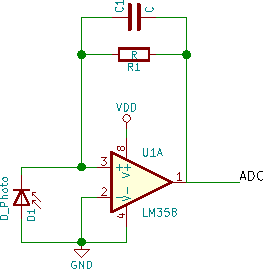
\includegraphics[width=9cm]{Circuit_Schematic.pdf}
	\caption{\label{fig:circuit}: Schematic of electronic circuit for photocurrent amplification. $V_{DD}$ is approximately $20V$. $D_1$ is a standard silicon photodiode, Hamamatsu part no. S1223-01. $R_1$ is valued at $\Omega$. The purpose of $C_1$ is to curb spontaneous oscillation at the output; its value is  . The amplifier is a dual-package PDIP LM358, a standard all-purpose operational amplifier. Its output is connected to a 14-bit ADC from National Instruments. Since all measurements presented here occur essentially at DC, no specific detail of this configuration is crucial.}
\end{figure}

\subsubsection{Beam re-sizing optics}

Though not depicted or mentioned in the main text, we use two conventional lenses, with focal lengths of roughly 50 and 25 mm, to shrink the beam-waist before illuminating the metasurface. Of course, with electron-beam lithography, there are constraints on the size of a metasurface that can ultimately be fabricated. Since the grating used for polarimetry is only $1.5$ mm $\times$ $1.5$ mm, we shrink the beam so that its entire extent may reside inside of the fabricated metasurface. Ideally, then, even if the beam moves around as polarization optics are rotated, it will remain inside of the metasurface.

We deliberately place the beam re-sizing lenses before the polarization optics that modify the polarization of the beam. Lenses may have some inherent, polarization-modifying stress-birefringence. Placing them before the final polarization optics allows us to neglect this, if it does exist. 

\subsection{Necessity of the polarizer following the grating}

In the main text, we present an design scheme for metasurface polarization gratings, that, when illuminated with a prescribed polarization state may produce desired states of polarization on its diffraction orders. By the reciprocity of polarization generators and analyzers, when the grating is used in reverse (that is, light passes through the grating and then a polarizer), the grating may also be used as a polarimeter.

Intuitively speaking, it might seem that the grating itself, without the inclusion of the linear polarizer, could function as a polarimeter alone. After all, as detailed in the main text, each grating order can be thought of as a diattenuator and a waveplate in series. As we detail here, these alone are not sufficient to form a full-Stokes polarimeter without the linear polarizer.

As detailed in the text, diffraction order $m$ may be thought of as having its own characteristic Jones matrix given by

\begin{equation}
	J_m = \begin{pmatrix}
	c_x^m & 0 \\ 0 & c_y^m
	\end{pmatrix}
	\begin{pmatrix}
	e^{i \delta_x^m} & 0 \\ 0 & e^{i \delta_y^m}
	\end{pmatrix}
\end{equation}

For a more general view of the behavior of the diffraction order, including its reponse to partially and un-polarized light, we must turn to the Mueller calculus, that is, the theory of $4\times4$ matrix operators on Stokes (rather than Jones) vectors \cite{Damask2005, Shurcliff1962}.

The Mueller matrix of a diattenuator oriented at $0\degree$ with respect to the $x$/$y$ coordinate system is given by

\begin{equation}
	\frac{1}{2}
	\begin{pmatrix}
	c_x^m + c_y^m & c_x^m - c_y^m & 0 & 0 \\
	c_x^m - c_y^m & c_x^m +c_y^m & 0 & 0 \\
	0 & 0 & 2\sqrt{c_x^m c_y^m} & 0 \\
	0 & 0 & 0 & 2\sqrt{c_x^m c_y^m}
	\end{pmatrix}
\end{equation}

where $c_x^m$ and $c_y^m$ are the amplitude transmission coefficients along $x$ and $y$. The Mueller matrix of a waveplate also oriented in this way is given by:

\begin{equation}
	\begin{pmatrix}
	1 & 0 & 0 & 0 \\	
	0 & 1 & 0 & 0 \\
	0 & 0 & \cos\delta_m & \sin\delta_m \\
	0 & 0 & -\sin\delta_m & \cos\delta_m
	\end{pmatrix}
\end{equation}

Here, $\delta_m = \delta_x^m - \delta_y^m$ is the retardance of the waveplate. 

The composite Mueller matrix of diffraction order $m$, then, is given by $M_m$, the product of the two above matrices:

\begin{equation}
	M_m =
	\frac{1}{2}
	\begin{pmatrix}
	c_x^m + c_y^m & c_x^m - c_y^m & 0 & 0 \\
	c_x^m - c_y^m & c_x^m +c_y^m & 0 & 0 \\
	0 & 0 & 2\cos\delta_m \sqrt{c_x^m c_y^m} & 2\sin\delta_m \sqrt{c_x^m c_y^m} \\
	0 & 0 & -2\sin\delta_m \sqrt{c_x^m c_y^m} & 2\cos\delta_m \sqrt{c_x^m c_y^m}
	\end{pmatrix}
\end{equation}

$M_m$ gives the full-polarization sensitive behavior of the combination of a diattenuator and waveplate on diffraction order $m$. What is truly of interest is the first row --- it is this row that dictates, for a given incident Stokes vector, what power will be measured at the output of the analyzer. If four such analyzers are placed on four diffraction orders, say $m=-2$, $-1$, $+1$, and $+2$, akin to the polarimeter compared here, we can immediately write the instrument matrix:

\begin{equation}
	A =
	\frac{1}{2}
	\begin{pmatrix}
	c_x^{-2} + c_y^{-2} & c_x^{-2} - c_y^{-2} & 0 & 0 \\
	c_x^{-1} + c_y^{-1} & c_x^{-1} - c_y^{-1} & 0 & 0 \\
	c_x^{+1} + c_y^{+1} & c_x^{+1} - c_y^{+1} & 0 & 0 \\
	c_x^{+2} + c_y^{+2} & c_x^{+2} - c_y^{+2} & 0 & 0 \\
	\end{pmatrix}
\end{equation}

By simple inspection, it is evident that the row-space of $A$ does not span $\mathbb{R}^4$ and we can immediately conclude that $\det A = 0$. Inversion is impossible, and this configuration cannot act as a full-Stokes polarimeter.

Let us consider a situation instead in which a polarizer is placed after the diattenuator/waveplate configuration. We allow the polarizer to take on a general orientation angle relative to $x$/$y$ which we denote $\theta$. Its Mueller matrix is:

\begin{equation}
	\frac{1}{2}
	\begin{pmatrix}
	1 & \cos2\theta & \sin2\theta & 0 \\
	\cos2\theta & \cos^2 2\theta & \sin2\theta \cos2\theta & 0 \\
	\sin2\theta & \sin2\theta \cos2\theta & \sin^2 2\theta & 0 \\
	0 & 0 & 0 & 2
	\end{pmatrix}
\end{equation}

If we then pre-multiply $M_m$ from above with the Mueller matrix of a polarizer oriented at $\theta$, we obtain the Mueller matrix:

\begin{equation}
	M_{m}' = \frac{1}{4}
	\begin{pmatrix}
	c_x^m + c_y^m + (c_x^m -c_y^m)\cos2\theta & c_x^m -c_y^m +(c_x^m +c_y^m) \cos 2\theta & 2\sqrt{c_x^m c_y^m} \cos\delta_m \sin 2\theta & 2\sqrt{c_x^m c_y^m}\sin\delta_m\sin 2\theta \\
	\cos2\theta (c_x^m + c_y^m + (c_x^m-c_y^m)\cos2\theta) &  \cos2\theta (c_x^m - c_y^m + (c_x^m+c_y^m)\cos2\theta) & \sqrt{c_x^m c_y^m} \cos\delta_m\sin 4\theta & sqrt{c_x^m c_y^m} \sin\delta_m\sin 4\theta \\
	(c_x^m +c_y^m +(c_x^m-c_y^m)\cos2\theta)\sin2\theta & (c_x^m -c_y^m +(c_x^m+c_y^m)\cos2\theta)\sin2\theta & 2\sqrt{c_x^m c_y^m} \cos\delta_m \sin^2 2\theta &   2\sqrt{c_x^m c_y^m} \sin\delta_m \sin^2 2\theta \\
	0 & 0 & -4\sqrt{c_x^m c_y^m} \sin\delta_m & 4\sqrt{c_x^m c_y^m} \cos\delta_m
	\end{pmatrix}
\end{equation}

Notably, the first row of this matrix has components in all four of its entries that are, in general, non-zero. An instrument matrix from four such analyzers, all sharing the same polarizer at the same orientation $\theta$:

\begin{equation}
A' =
	\begin{pmatrix}
	c_x^{-2} + c_y^{-2} + (c_x^{-2} -c_y^{-2})\cos2\theta & c_x^{-2} -c_y^{-2} +(c_x^{-2} +c_y^{-2}) \cos 2\theta & 2\sqrt{c_x^{-2} c_y^{-2}} \cos\delta_{-2} \sin 2\theta & 2\sqrt{c_x^{-2} c_y^{-2}}\sin\delta_{-2}\sin 2\theta \\
	c_x^{-1} + c_y^{-1} + (c_x^{-1} -c_y^{-1})\cos2\theta & c_x^{-1} -c_y^{-1} +(c_x^{-1} +c_y^{-1}) \cos 2\theta & 2\sqrt{c_x^{-1} c_y^{-1}} \cos\delta_{-1} \sin 2\theta & 2\sqrt{c_x^{-1} c_y^{-1}}\sin\delta_{-1}\sin 2\theta \\
	c_x^{+1} + c_y^{+1} + (c_x^{+1} -c_y^{+1})\cos2\theta & c_x^{+1} -c_y^{+1} +(c_x^{+1} +c_y^{+1}) \cos 2\theta & 2\sqrt{c_x^{+1} c_y^{+1}} \cos\delta_{+1} \sin 2\theta & 2\sqrt{c_x^{+1} c_y^{+1}}\sin\delta_{+1}\sin 2\theta \\
	c_x^{+2} + c_y^{+2} + (c_x^{+2} -c_y^{+2})\cos2\theta & c_x^{+2} -c_y^{+2} +(c_x^{+2} +c_y^{+2}) \cos 2\theta & 2\sqrt{c_x^{+2} c_y^{+2}} \cos\delta_{+2} \sin 2\theta & 2\sqrt{c_x^{+2} c_y^{+2}}\sin\delta_{+2}\sin 2\theta
	\end{pmatrix}
\end{equation}

There are suitable choices of the $\{c_x^m\}$, $\{c_y^m\}$, and $\{\delta_m\}$ such that $A'$ is invertible.


\subsection{Calibration procedure, step-by-step}

In this section we detail the calibration procedure used to calibrate the metasurface polarimeter in a very deliberate manner. We hope that this can serve as a helpful guide for others approaching this problem for the first time.

Credit for this calibration procedure, which distinguishes itself by explicitly allowing for imperfect waveplate optics, ultimately lies with Azzam and colleagues \citep{Azzam1989}. However, the process used here is in some respects a modification of that presented in \cite{Azzam1989}.

\subsubsection{Linear polarizer only}

\begin{figure}[!htp]
	\centering
	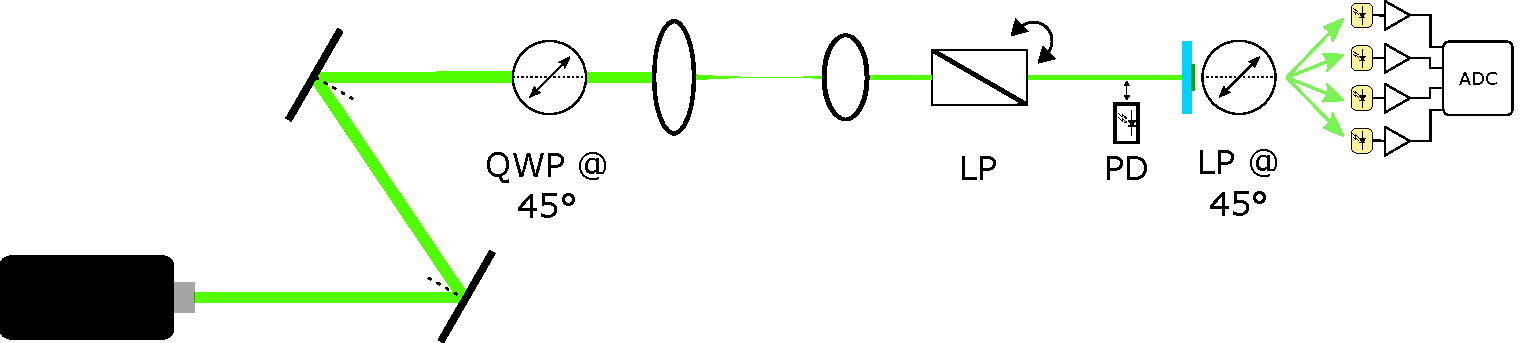
\includegraphics[width=\linewidth]{schematic_I.pdf}
	\caption{\label{fig:schematic_I}: Schematic of the optical setup used during the first step of the calibration of the metasurface grating polarimeter.}
\end{figure}

Following \citep{Azzam1989}, we may write the instrument matrix to-be-determined in terms of its columns:

\begin{equation}
A = \begin{pmatrix}
| & | & | & | \\
\vec{A}_0 & \vec{A}_1 & \vec{A}_2 & \vec{A}_3 \\
| & | & | & |
\end{pmatrix}
\end{equation}

In this first calibration step, the polarization incident on the meta-grating polarimeter is set by a single linear polarizer (Glan-Thompson). When the linear polarizer is oriented at an angle $\theta$, it produces a Stokes vector given by $\vec{S}(\theta) = \begin{bmatrix} 1 & \cos2\theta & \sin2\theta & 0 \end{bmatrix}^T$ assuming that the power of the incident beam is unity. Then, the intensity vector (that is, the list of intensities measured on the four photodiodes) is given by $A\vec{S}(\theta)$:

\begin{equation}
	\label{eqn:intensity}
	\vec{I} = \vec{A}_0 + \vec{A}_1 \cos2\theta + \vec{A}_2 \sin 2\theta
\end{equation} 

As we vary the incident linear polarization, we can record the values on each of the four channels. We can normalize these values by the incident beam power $i_{\theta}$ and plot against $\theta$.

This yields four sinusoidal curves. By fitting the curves to the functional form of Eqn. \ref{eqn:intensity}, we may obtain the first three columns of the instrument matrix (that is, $\vec{A}_0$, $\vec{A}_1$, and $\vec{A}_2$).

In Fig. \ref{fig:schematic_I}, the optical setup during this first stage of calibration is shown. Light from the laser source at $\lambda=532$ nm bounces off two alignment mirrors and passes through a quarter-waveplate (as discussed above) to compensate for the preferred linear polarization of the laser source. It passes through two beam reduction lenses so that its spatial extent may fit inside the square boundaries of the 1.5 mm $\times$ 1.5 mm metasurface polarization grating. After being polarized by a Glan-Thompson linear polarizer, light passes through the metasurface diffraction grating and is split into many diffraction orders, the central four of which pass through a fixed linear polarizer at $45\degree$ and then impinge upon four photodiodes, whose values are amplified and recorded on a computer.

The linear polarizer is placed in a motorized rotation mount and its orientation is varied in $5\degree$ steps. At each step, a photodiode swings in front of the beam (blocking it), records the beam power, and then swings back out in an automated fashion in order to obtain the incident beam power $i_{\theta}$. Additionally, for every $\theta$, we measure the power reported by the four photodiodes directly following the metasurface.

It should be noted that this first calibration step introduces a coordinate system to the polarimeter --- the $\theta = 0\degree$ point of the linear polarizer becomes the origin of the polarimeter's angular coordinate system. This need not be necessarily well-aligned with the optical table or any external coordinate frame.

\textbf{Experimental tip:} We found that, as the linear polarizer rotated, we could very visibly observe that its trajectory on the metasurface sample moved around in a circular orbit, of sorts (as in Fig. \ref{fig:orbit}). At times, the incident beam would near the edge of the sample. We found that this ``orbiting" effect compromised our measurements and would severely skew the sinusoidal calibration curves. In order to allow ourselves freedom to correct this effect, we mounted the Glan-Thompson polarizer in a tip/tilt mount before placing it in a motorized rotation mount. Then, we would set the rotation mount to rotate at a constant angular velocity and observe the aforementioned ``orbit" effect and correct the tip/tilt of the polarizer until it was eliminated.

We were not able to reliably identify the source of this effect. We suspect that the Glan-Thompson, being a prism polarizer, may suffer from some misalignment of the two prisms relative to one another. Consequently, there would be a refraction at the middle interface.

\begin{figure}[!htp]
	\centering
	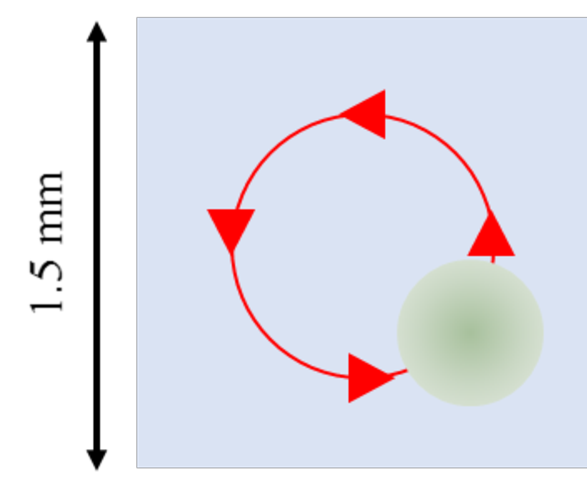
\includegraphics[width=5cm]{orbit.pdf}
	\caption{\label{fig:orbit}: Visualization: As the linear polarizer is rotated, the incident laser beam traces out a circular path on the metasurface.}
\end{figure} 

\subsubsection{Linear polarizer and quater-waveplate}

\begin{figure}[!htp]
	\centering
	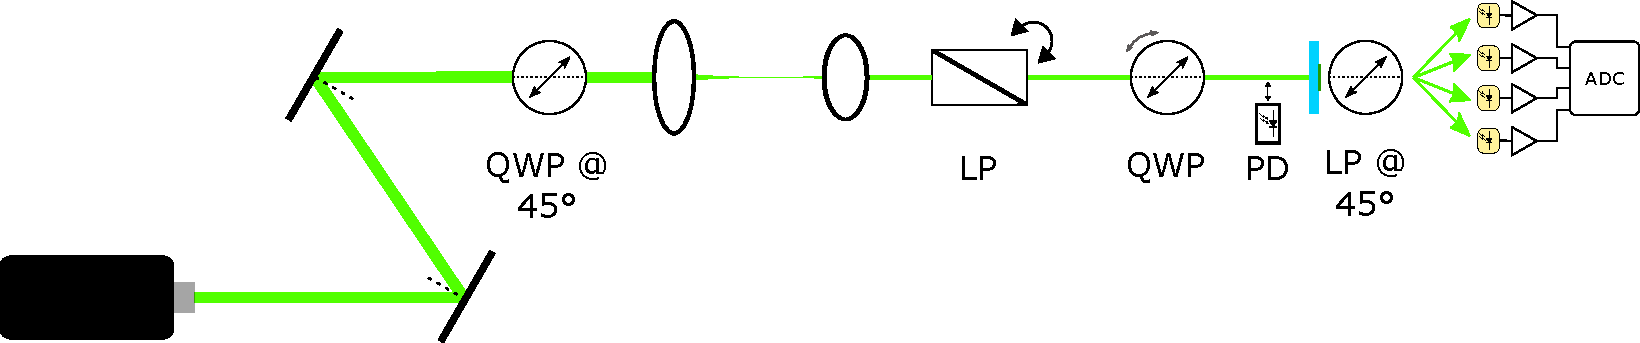
\includegraphics[width=\linewidth]{schematic_II.pdf}
	\caption{\label{fig:schematic_II}: Schematic of the optical setup used during the second step of the calibration of the metasurface grating polarimeter.}
\end{figure}

\begin{figure}[!htp]
	\centering
	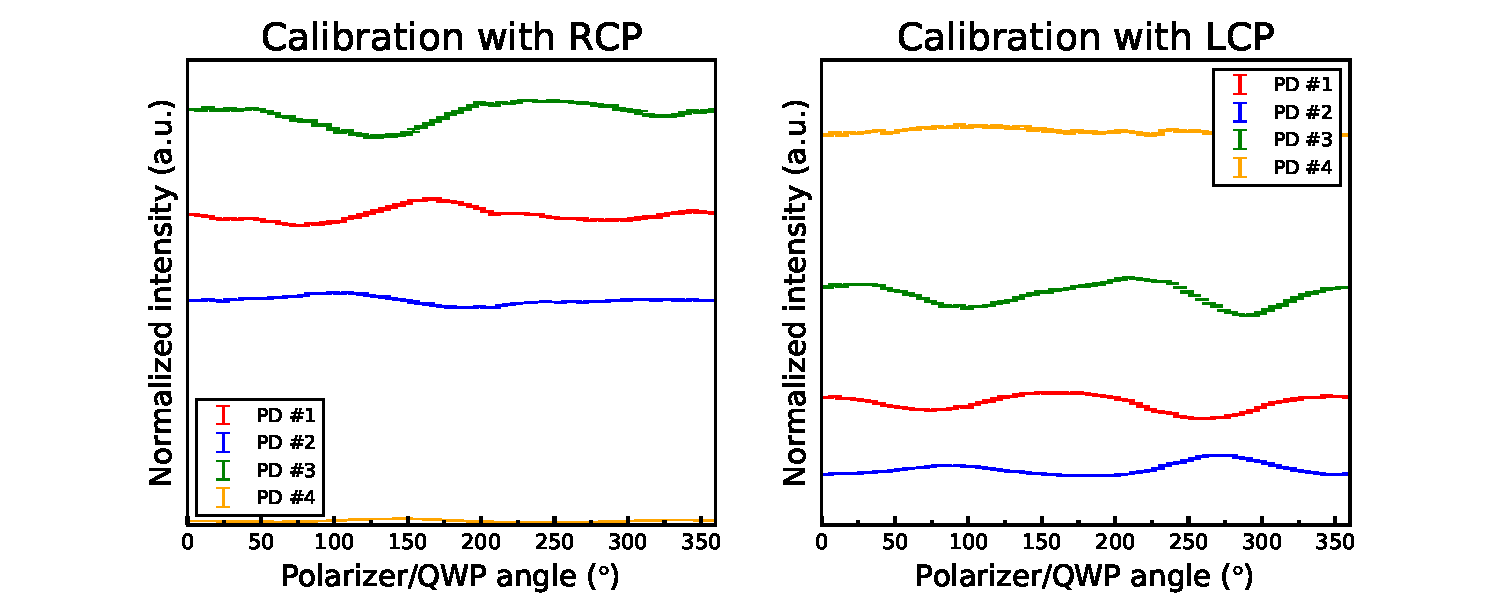
\includegraphics[width=\linewidth]{qwp_cal.pdf}
	\caption{\label{fig:qwp_cal}: Calibration data obtained from the exposing the polarimeter to RCP and LCP light. Averaging the values obtained on each channel yields $\vec{I}_{\text{RCP}}$ and $\vec{I}_{\text{LCP}}$. Note that for one circular polarization, Photodiode 1 is nearly extinguished, while for the other it is maximal, as would be expected from the designed polarization state.}
\end{figure}

With only a linear polarizer, the first three columns of the instrument matrix are easily determined. The last column requires test polarization states with some chirality.

Circularly polarized light has a Stokes vector given by $\begin{bmatrix}
1 & 0 & 0 & \pm 1
\end{bmatrix}^T$, where the $\pm$ distinguishes between right- and left-handed circular polarization. As shown in \citep{Azzam1989}, the last column of the instrument matrix may be written as

\begin{equation}
\label{eqn:A3}
\vec{A}_3 = \frac{1}{2} (\vec{I}_{\text{RCP}} - \vec{I}_{\text{LCP}})
\end{equation}

We must, then, obtain the (incident intensity normalized) values of the readings on all four photodiodes when exposed to each circular polarization. This presents a problem however; as detailed above, production of perfect circular polarization --- at least with off-the-shelf waveplates --- 
is nearly impossible.

Azzam presents a solution \citep{Azzam1989}, so long as the retardance of the waveplate is nearly a quarter-wave, that is, so long as it deviates from $90\degree$ by a small angle. A linear polarization and a quarter-waveplate oriented at $45\degree$ relative to one another produce \textit{nearly} circular polarization. If both the polarizer and the waveplate are rotated together by $90\degree$, the same nearly-circular elliptical polarization will be produced, but rotated by $90\degree$. To first order, the effect of averaging the polarimeter's readings when exposed to both configurations is the same as if perfect circular polarization were available.

In Azzam's original scheme, this average contains only two data points, at $0\degree$ and $90\degree$. In the present work, we take many such data points between $0\degree$ and $360\degree$ in order to decrease error.

In the experiment, as depicted in Fig. \ref{fig:schematic_II}, both a linear polarizer and a quarter-waveplate are placed in the beampath in front of the metasurface grating polarimeter. Both are controlled with automated rotation mounts. When the quarter-waveplate is inserted, the angular position of its fast axis must be determined. A second Glan-Thompson polarizer is placed in front of the first, and the first polarizer is rotated until the intensity of the beam is nulled (the polarizers are crossed). Then, the quarter-waveplate is inserted between the two, and angular position at which the intensity transmitted through the polarizer-waveplate-polarizer configuration is maximized. This should be where the fast axis is at $45\degree$ relative to the first polarizer. This position is determined by testing the transmitted intensity at many angular locations and fitting a trigonmetric function to find the location of the maximum.

Next, the second polarizer is removed, so that only the first polarizer and the waveplate oriented at a relative angle of $45\degree$ remain. The polarizer/waveplate combination is rotated in tandem in $5\degree$ increments and at each configuration, the intensities on the four photodiodes are recorded. In addition, the power of the incident beam $i_{\theta}$ is also recorded in each configuration by a photodiode that moves in and out of the beam.

For each of the four photodiodes, the normalized intensities measured at each $\theta$ are computed. These are averaged together to form the vector $\vec{I}_{\text{RCP}}$.  Then, the quarter-waveplate is rotated by $90\degree$, and the entire process above is repeated to obtain the vector $\vec{I}_{\text{LCP}}$.

This data is depicted in Fig. \ref{fig:qwp_cal}. It is of note that for incident RCP light, the intensity on PD \# 4 is very low, while for LCP the case is reversed. This confirms that, indeed, one of the diffraction orders produces near-circularly polarized light, as desired. Second, we note that the values on each photodiode vary as the linear polarizer/QWP combination is rotated. This is to be expected to a certain extent, since the polarization is not exactly circular. One would expect, however, that the variation would be sinusoidal in nature. Despite our best efforts, we cannot account for the skewed shape of these curves; we suspect that it may have something to do with the orbiting effect of Fig. \ref{fig:orbit}.

\subsubsection{Compilation of the instrument matrix}

Finally, the instrument matrix can be assembled --- the first three columns can be drawn from the linear polarization-only measurements, while the last column can be computed from $\vec{I}_{\text{RCP}}$ and $\vec{I}_{\text{LCP}}$ cf. Eqn. \ref{eqn:A3}.

\subsection{Production of partially polarized light}

Full-Stokes polarimetry, as its name connotes, allows for the determination of the entire Stokes vector. This allows for the analysis of partially polarized beams of light, for which the degree of polarization $p$ may be less than unity.

In general, a partially polarized beam must have a spectral bandwidth $\Delta \omega$ sufficiently large such that its time-bandwidth product $\tau \Delta \omega \gg 1$, where $\tau$ is the mean optical period of the wavepacket.

\subsection{Error propagation and error bars}

\begin{itemize}
\item Hello, world!
\end{itemize}

\subsection{Comment on the commercial rotating waveplate polarimeter (RWP)}

\section{Angle dependence of polarization production and polarimetry}

\subsection{Effect of off-normal incidence on the produced polarization ellipses}

\subsection{Effect of off-normal incidence on polarimeter calibration and Stokes vector determination}



% If in two-column mode, this environment will change to single-column
% format so that long equations can be displayed. Use
% sparingly.
%\begin{widetext}
% put long equation here
%\end{widetext}

% figures should be put into the text as floats.
% Use the graphics or graphicx packages (distributed with LaTeX2e)
% and the \includegraphics macro defined in those packages.
% See the LaTeX Graphics Companion by Michel Goosens, Sebastian Rahtz,
% and Frank Mittelbach for instance.
%
% Here is an example of the general form of a figure:
% Fill in the caption in the braces of the \caption{} command. Put the label
% that you will use with \ref{} command in the braces of the \label{} command.
% Use the figure* environment if the figure should span across the
% entire page. There is no need to do explicit centering.

% \begin{figure}
% \includegraphics{}%
% \caption{\label{}}
% \end{figure}

% Surround figure environment with turnpage environment for landscape
% figure
% \begin{turnpage}
% \begin{figure}
% \includegraphics{}%
% \caption{\label{}}
% \end{figure}
% \end{turnpage}

% tables should appear as floats within the text
%
% Here is an example of the general form of a table:
% Fill in the caption in the braces of the \caption{} command. Put the label
% that you will use with \ref{} command in the braces of the \label{} command.
% Insert the column specifiers (l, r, c, d, etc.) in the empty braces of the
% \begin{tabular}{} command.
% The ruledtabular enviroment adds doubled rules to table and sets a
% reasonable default table settings.
% Use the table* environment to get a full-width table in two-column
% Add \usepackage{longtable} and the longtable (or longtable*}
% environment for nicely formatted long tables. Or use the the [H]
% placement option to break a long table (with less control than 
% in longtable).
% \begin{table}%[H] add [H] placement to break table across pages
% \caption{\label{}}
% \begin{ruledtabular}
% \begin{tabular}{}
% Lines of table here ending with \\
% \end{tabular}
% \end{ruledtabular}
% \end{table}

% Surround table environment with turnpage environment for landscape
% table
% \begin{turnpage}
% \begin{table}
% \caption{\label{}}
% \begin{ruledtabular}
% \begin{tabular}{}
% \end{tabular}
% \end{ruledtabular}
% \end{table}
% \end{turnpage}

% Specify following sections are appendices. Use \appendix* if there
% only one appendix.
%\appendix
%\section{}

% If you have acknowledgments, this puts in the proper section head.
%\begin{acknowledgments}
% put your acknowledgments here.
%\end{acknowledgments}

% Create the reference section using BibTeX:
\bibliography{Polarimetry_and_metasurface_polarization.bib}


\end{document}
%
% ****** End of file apstemplate.tex ******
